% ==============================================================================
% LAB 119
% UNDERSÖKNING AV RC-KRETS
% ------------------------
%
% Author:
% Jonas Sjöberg     <tel12jsg@student.hig.se>
% Oscar Wallberg    <tco13owg@student.hig.se>
%
% License:
% Creative Commons Attribution-NonCommercial-ShareAlike 4.0 International
% See LICENSE.md for full licensing information.
% ==============================================================================

\documentclass[11pt,a4paper]{article}
\usepackage[utf8]{inputenc}
\usepackage[swedish]{babel}         % För svensk innehållsförteckning
\usepackage[swedish]{isodate}
\usepackage{siunitx}                % (För dokumentation, kör; texdoc siunitx)
\usepackage{amssymb}
\usepackage{amsmath}
\usepackage{amsfonts}
\usepackage{graphicx}
\usepackage{booktabs}
\usepackage{longtable}              % Tables span across pages
\usepackage{microtype}
\usepackage{gensymb}
%\usepackage{tabto}
\usepackage{units}
\setlength\parindent{0pt}           % Removes all indentation from paragraphs

\usepackage{rotating}
\usepackage{wrapfig}
\usepackage{lscape}

\usepackage[pdfusetitle,
            bookmarks=true,
            bookmarksnumbered=true,
            bookmarksopen=false,
            breaklinks=false,
            pdfborder={0 0 0},
            backref=false,
            colorlinks=false]{hyperref}


\title{EE466 \\ Lab 119 \\ Undersökning av RC-krets}

\author{                                 \\
  Jonas Sjöberg                          \\
  860224                                 \\
  Högskolan i Gävle,                     \\
  Elektronikingenjörsprogrammet,         \\
  \texttt{tel12jsg@student.hig.se}       \\
  \texttt{https://github.com/jonasjberg} \\
                                         \\
  Oscar Wallberg                         \\
  Högskolan i Gävle,                     \\
  Dataingenjörsprogrammet,               \\
  \texttt{tco13owg@student.hig.se}       \\
}

\date{}

\begin{document}
\maketitle

\begin{center}
  \begin{tabular}{l r}
    Labb utförd: & TODO: Labben utförd datum \\
    Instruktör:  & Efrain Zenteno
  \end{tabular}
\end{center}

\medskip

\begin{abstract}
  \begin{center}
    Laborationsrapport för \emph{EE466 -- Elektrisk kretsteori}, Högskolan i
    Gävle. Syftet med laborationen är att analysera funktionen hos en RC krets.
    Laborationen innefattar överföringsfunktionen för en RC-krets, i både tids-
    och frekvensdomänen. Stegsvaret för en första ordningens krets.
    Bode-diagram.  Begreppen brytfrekvens, frekvens- och faskaraktäristik.
  \end{center}
\end{abstract}

\newpage
%\hypersetup{linkcolor=black}
\setcounter{tocdepth}{3}
\tableofcontents

\newpage
% ==============================================================================
% LAB 119
% UNDERSÖKNING AV RC-KRETS
% ------------------------
%
% Author:
% Jonas Sjöberg     <tel12jsg@student.hig.se>
% Oscar Wallberg    <tco13owg@student.hig.se>
%
% License:
% Creative Commons Attribution-NonCommercial-ShareAlike 4.0 International
% See LICENSE.md for full licensing information.
% ==============================================================================

\section{Introduktion}\label{intro}
I denna labb skall vi studera en passiv krets uppbyggd av ett motstånd och en
kondensator. Om en sådan krets matas med en sinusformad insignal kommer den att
släppa igenom vissa frekvenser medan andra frekvenser dämpas. Ett sådant
frekvensberoende nät kallas därför ofta för filter. Om kretsen innehåller
endast en reaktiv (dvs energilagrande) komponent (spole eller kondensator)
kallar vi kretsen för ett första ordningens filter. Namnet kommer sig av att
kretsen kan beskrivas med en första ordningens differentialekvation.
Vi skall analysera kretsen både i frekvensplanet genom att mäta upp ett
Bode-diagram och i tidsplanet genom att mäta upp kretsens stegsvar.


% ==============================================================================
% LAB 119
% UNDERSÖKNING AV RC-KRETS
% ------------------------
%
% Author:
% Jonas Sjöberg     <tel12jsg@student.hig.se>
%
% License:
% Creative Commons Attribution-NonCommercial-ShareAlike 4.0 International
% See LICENSE.md for full licensing information.
% ==============================================================================

\section{Uppmätning av Bode-diagram}\label{bode}
\subsection{Beräkning}
% ------------------------------------------------------------------------------
Brytfrekvensen $f_1$ defineras som den frekvens då signalen har dämpats med
\SI{3}{\dB} och beräknas från ekv.~\eqref{eq:transfer2} enligt:

\begin{equation}\label{eq:cutoff}
  f_1 = \dfrac{1}{2 \pi R C} \si{\Hz}
\end{equation}

För kopplingen med komponentvärden enligt Figur~\ref{fig:rc-schema} beräknas
brytfrekvensen $f_1$ enligt ekv.~\eqref{eq:cutoff2}:

\begin{equation}\label{eq:cutoff2}
  \begin{split}
    f_1 &= \dfrac{1}{2 \pi \times \SI{1}{\kohm} \times \SI{100}{\nano\farad}} \si{\Hz} \\
        &= \dfrac{1}{2 \pi \times \num{1e3} \times \num{100e-6}} \si{\Hz}              \\
        &= \dfrac{10^6}{2 \pi \times 10^3 \times \num{100}} \si{\Hz}                   \\
    f_1 &= \SI{1.591549431}{\kHz}
  \end{split}
\end{equation}

Vilket ger svaret i \eqref{eq:cutoff3}; signalen dämpas med \SI{3}{\dB} vid
filtrets brytfrekvens $f_1 \approx \SI{1.592}{\kHz}$, varvid den ``rullas av''
med \SI{20}{\dB} per dekad (frekvenshöjning med en faktor av 10).

\begin{equation}\label{eq:cutoff3}
  \begin{split}
    f_1 &= \SI{1.591549431}{\kHz} \\
    f_1 &\approx \SI{1.592}{\kHz} \\
  \end{split}
\end{equation}


\subsection{Genomförande}
% ------------------------------------------------------------------------------
Genomförandet av mätningar visas i Figur~\ref{fig:bode-foto-1000},
Figur~\ref{fig:bode-foto-1300}, Figur~\ref{fig:bode-foto-1500},
Figur~\ref{fig:bode-foto-1800}, Figur~\ref{fig:bode-foto-1900} samt
Figur~\ref{fig:bode-foto-2000}.


\begin{figure}
  \centering
  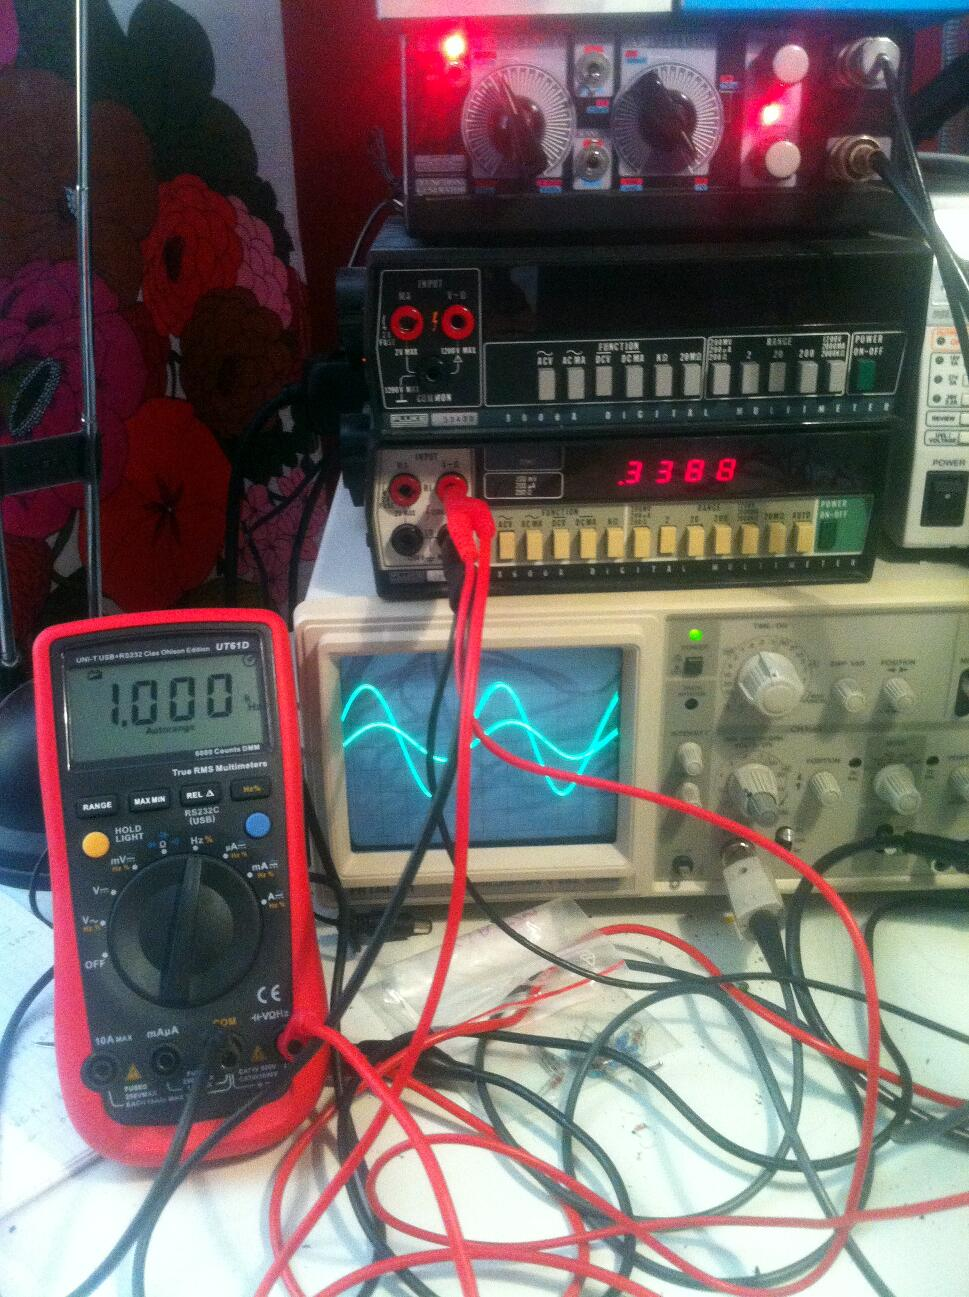
\includegraphics[width=\linewidth]{img/bode_1000Hz.jpg}
  \caption[] {Mätningar av data presenterade i Tabell~\ref{table-bode}.
              Signalfrekvens \SI{1}{\kHz}}.
  \label{fig:bode-foto-1000}
\end{figure}

\begin{figure}
  \centering
  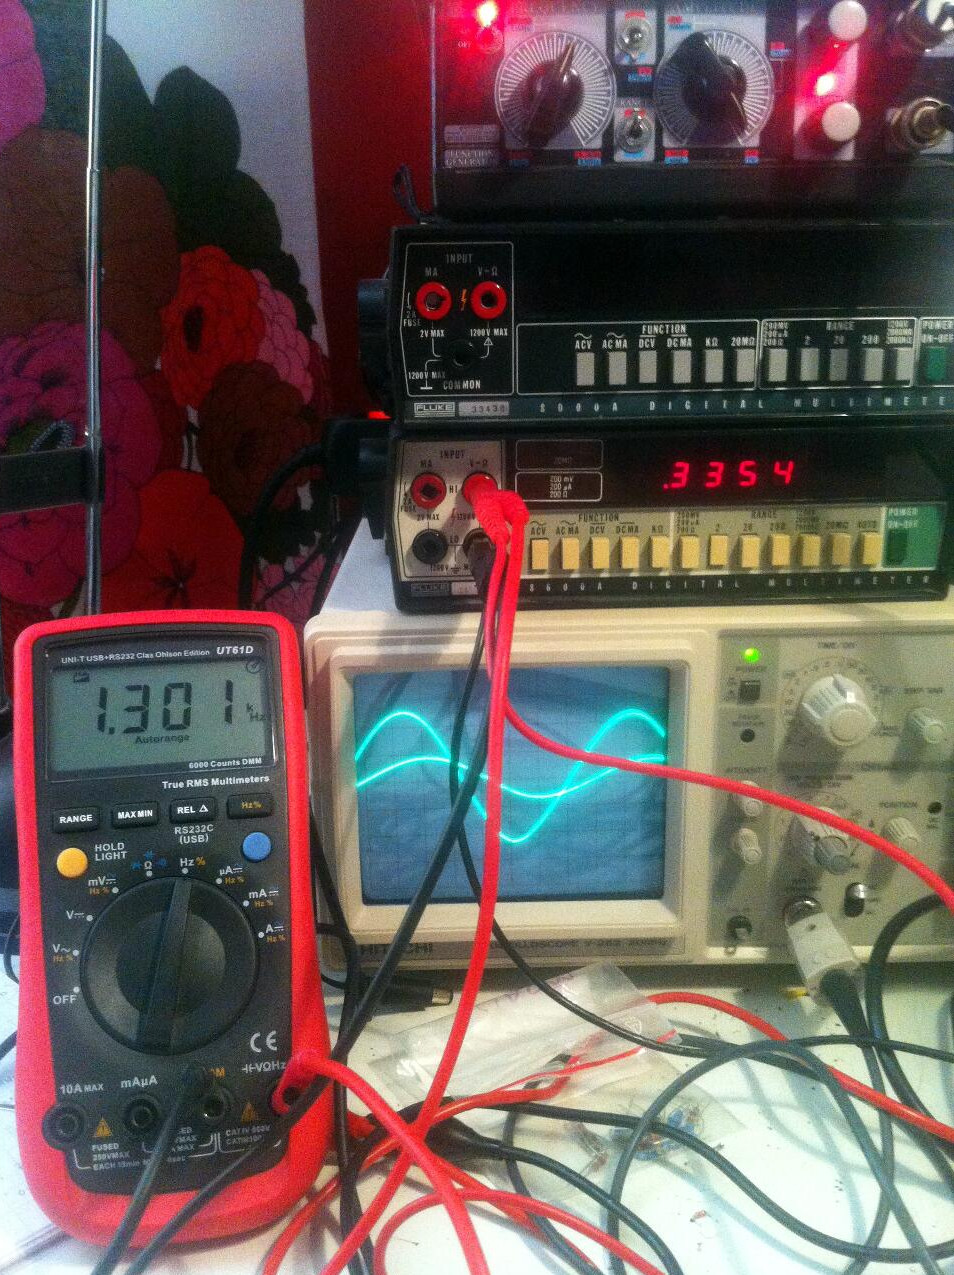
\includegraphics[width=\linewidth]{img/bode_1300Hz.jpg}
  \caption[] {Mätningar av data presenterade i Tabell~\ref{table-bode}.
              Signalfrekvens \SI{1.3}{\kHz}}.
  \label{fig:bode-foto-1300}
\end{figure}

\begin{figure}
  \centering
  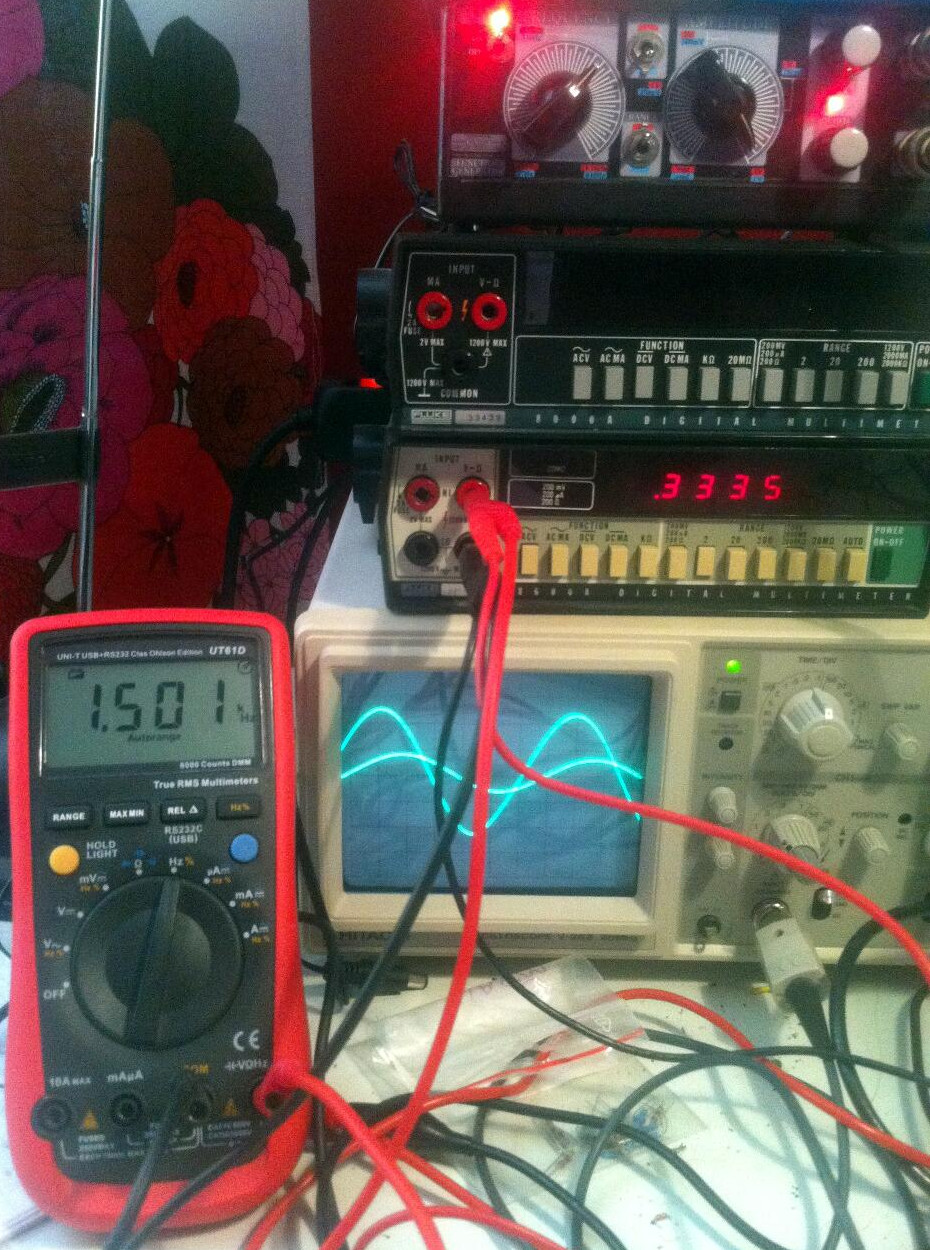
\includegraphics[width=\linewidth]{img/bode_1500Hz.jpg}
  \caption[] {Mätningar av data presenterade i Tabell~\ref{table-bode}.
              Signalfrekvens \SI{1.5}{\kHz}}.
  \label{fig:bode-foto-1500}
\end{figure}

\begin{figure}
  \centering
  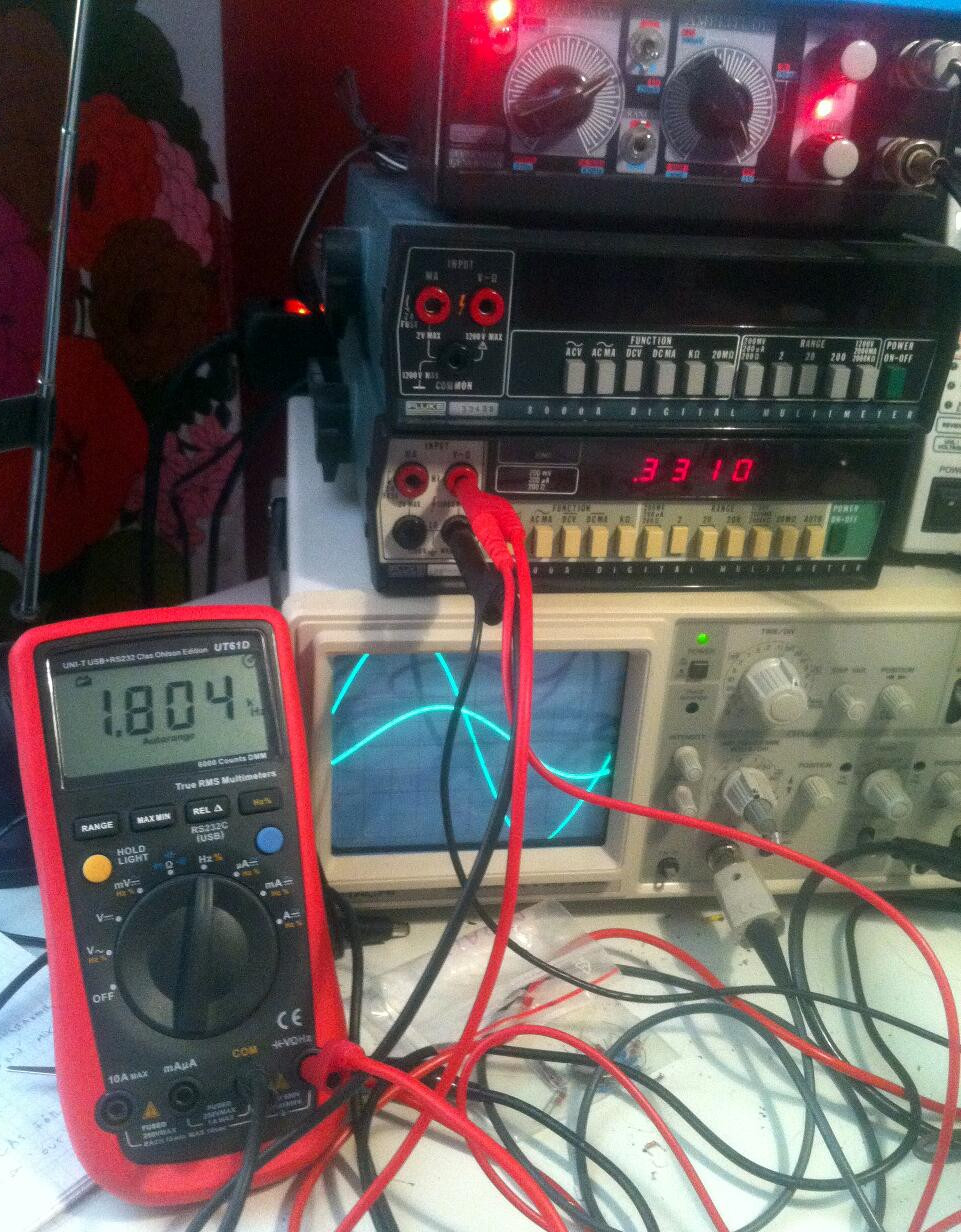
\includegraphics[width=\linewidth]{img/bode_1800Hz.jpg}
  \caption[] {Mätningar av data presenterade i Tabell~\ref{table-bode}.
              Signalfrekvens \SI{1.8}{\kHz}}.
  \label{fig:bode-foto-1800}
\end{figure}

\begin{figure}
  \centering
  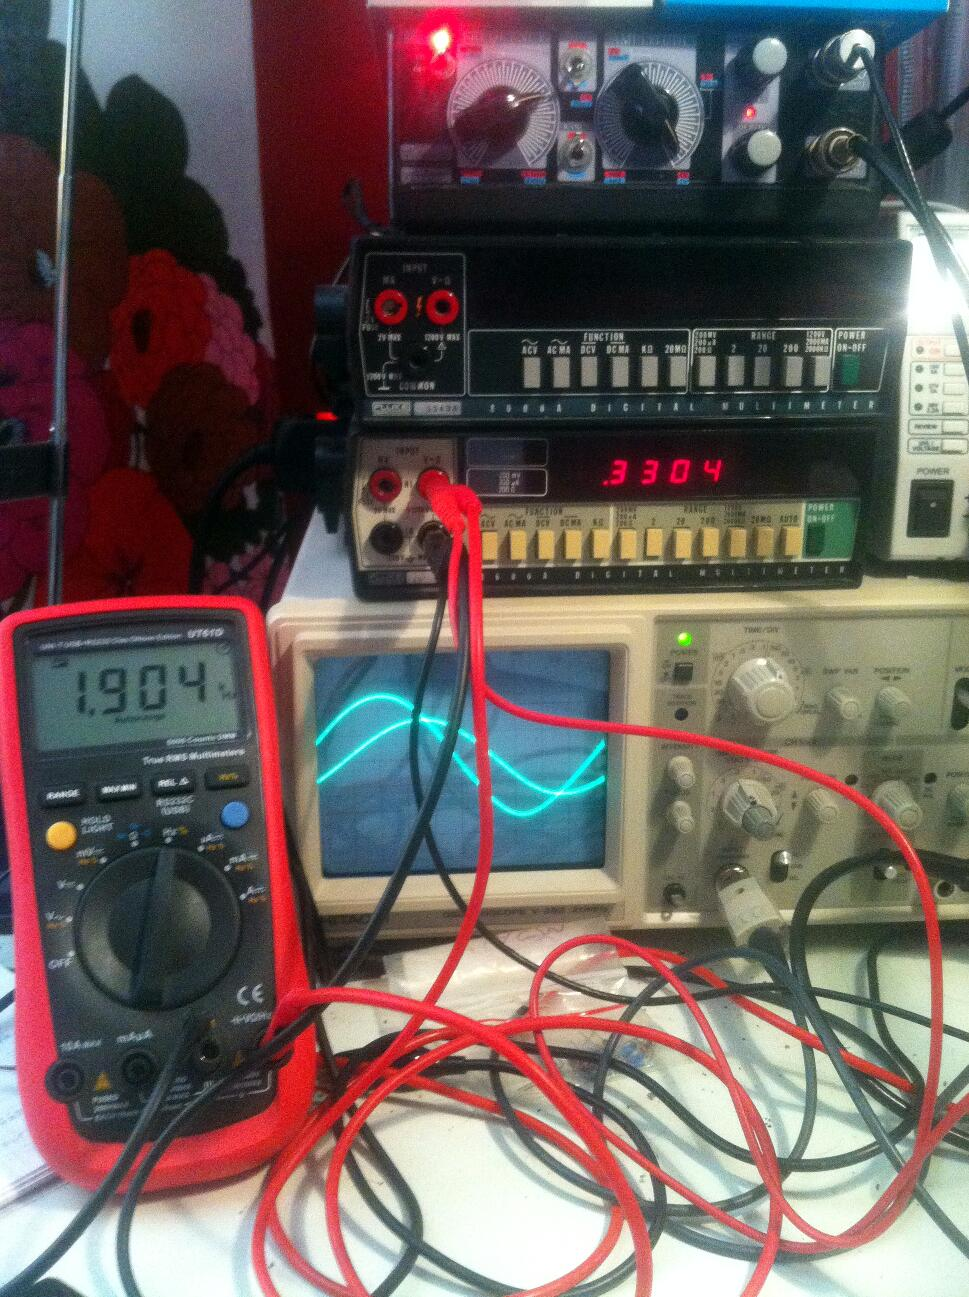
\includegraphics[width=\linewidth]{img/bode_1900Hz.jpg}
  \caption[] {Mätningar av data presenterade i Tabell~\ref{table-bode}.
              Signalfrekvens \SI{1.9}{\kHz}}.
  \label{fig:bode-foto-1900}
\end{figure}

\begin{figure}
  \centering
  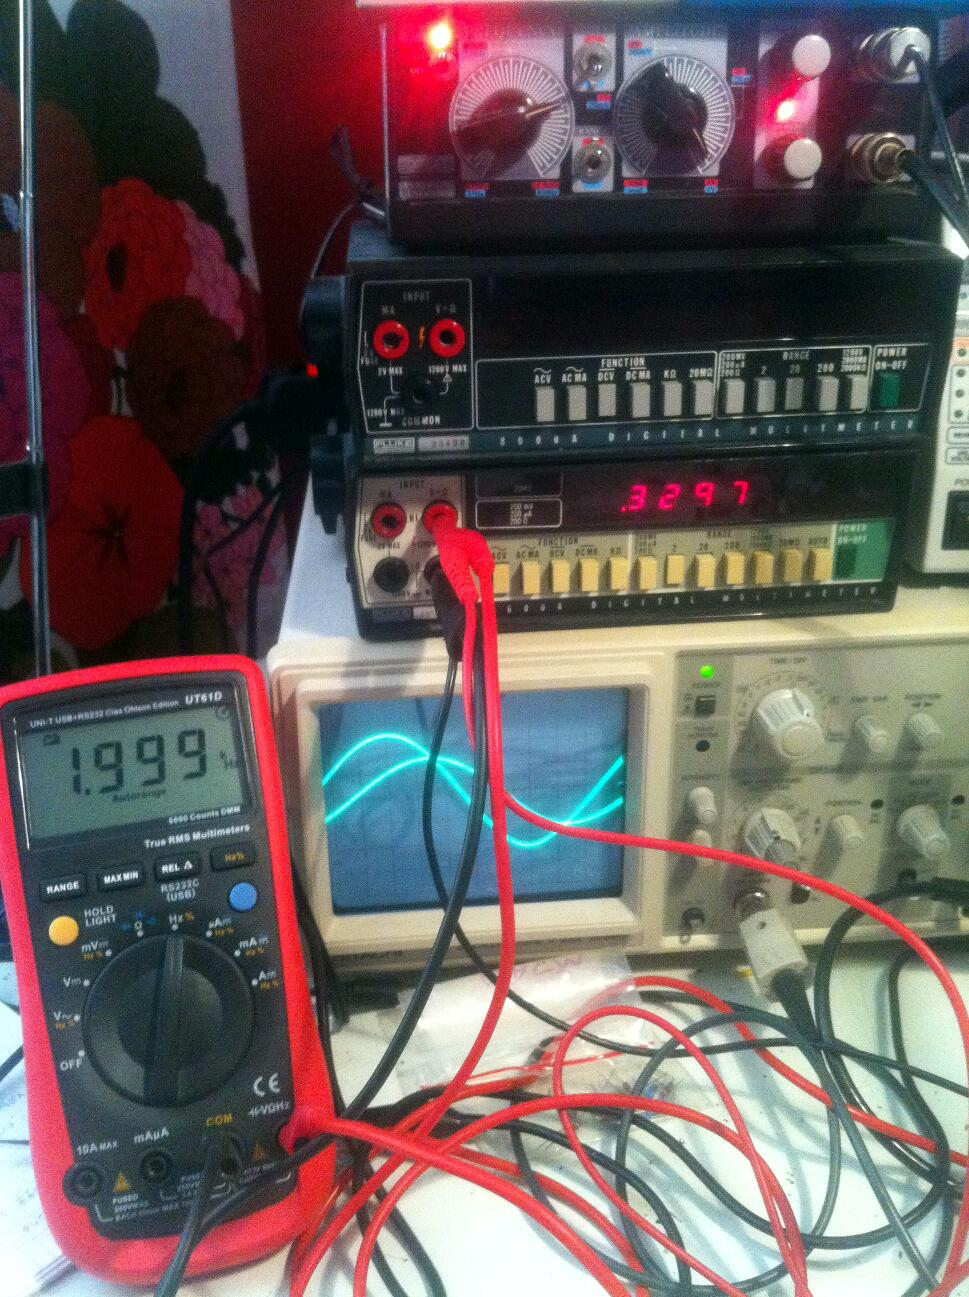
\includegraphics[width=\linewidth]{img/bode_2000Hz.jpg}
  \caption[] {Mätningar av data presenterade i Tabell~\ref{table-bode}.
              Signalfrekvens \SI{2}{\kHz}}.
  \label{fig:bode-foto-2000}
\end{figure}


\subsection{Mätresultat}
% ------------------------------------------------------------------------------
Mätresultaten presenteras i Tabell~\ref{table-bode}.

\begin{longtable}[c]{@{}ccccc@{}}
  \toprule\addlinespace
    \begin{tabular}{cc}$\text{Frekvens}        \\ (\si{\hertz})$   \end{tabular}
  & \begin{tabular}{cc}$U_{ut}                 \\ (\si{\volt})$    \end{tabular}
  & \begin{tabular}{cc}$U_{ut}/U_{in}          \\ (\si{\volt})$    \end{tabular}
  & \begin{tabular}{cc}$20 \log{U_{ut}/U_{in}} \\ (\si{\dB})$      \end{tabular}
  & \begin{tabular}{cc}$\phi                   \\ \text{(grader)}$ \end{tabular}
  \\\addlinespace
  \midrule\endhead
   100 & 1.004 & 1.004 & \SI{ 34.67}{\milli} & -3.6 \\\addlinespace
   200 & 0.998 & 0.998 & \SI{-17.38}{\milli} & -7.2 \\\addlinespace
   300 & 0.997 & 0.997 & \SI{-26.09}{\milli} & -10  \\\addlinespace % 1mS
   500 & 0.990 & 0.990 & \SI{-87.29}{\milli} & -17  \\\addlinespace % 0.1mS   ???
   700 & 0.984 & 0.984 & \SI{-140.1}{\milli} & -23  \\\addlinespace % 0.15mS  ???
  1000 & 0.958 & 0.958 & \SI{-372.7}{\milli} & -32  \\\addlinespace % 0.1mS   ???
  1200 & 0.952 & 0.952 & \SI{-427.3}{\milli} & -37  \\\addlinespace % 60uS
  1300 & 0.949 & 0.949 & \SI{-454.7}{\milli} & -39  \\\addlinespace % ????
  1500 & 0.943 & 0.943 & \SI{-509.8}{\milli} & -43  \\\addlinespace % 40uS
  1600 & 0.940 & 0.940 & \SI{-537.4}{\milli} & -45  \\\addlinespace % 35uS
  1700 & 0.938 & 0.938 & \SI{-555.9}{\milli} & -47  \\\addlinespace % ?????
  1800 & 0.936 & 0.936 & \SI{-574.5}{\milli} & -48  \\\addlinespace % 35uS
  1900 & 0.934 & 0.934 & \SI{-593.1}{\milli} & -50  \\\addlinespace % 35uS
  2000 & 0.932 & 0.932 & \SI{-611.7}{\milli} & -51  \\\addlinespace % ????
  \bottomrule
  \addlinespace
  \caption[]{Mätresultat för kretsen i Figur~\ref{fig:rc-schema}.}
  \label{table-bode}
\end{longtable}


% TODO: Bode-diagram för frekvensgång.

% TODO: Bode-diagram för Fasförskjutning.


\subsection{Simulering}
% ------------------------------------------------------------------------------
För verifiering och visualisering av den teoretiska beräkningen körs en
\texttt{SPICE}-simulering av kretsen i det GPL-licensierade open source
programmet \texttt{Qucs}\footnote{\url{http://qucs.sourceforge.net/}}.
Simuleringsuppställningen och resultatet återfinns i
Figurer~\ref{fig:bode-sim-ac}, Figur~\ref{fig:bode-sim-tran} och
Figur~\ref{fig:bode-sim-param}.

\begin{figure}\label{fig:bode-sim-ac}
  \centering
  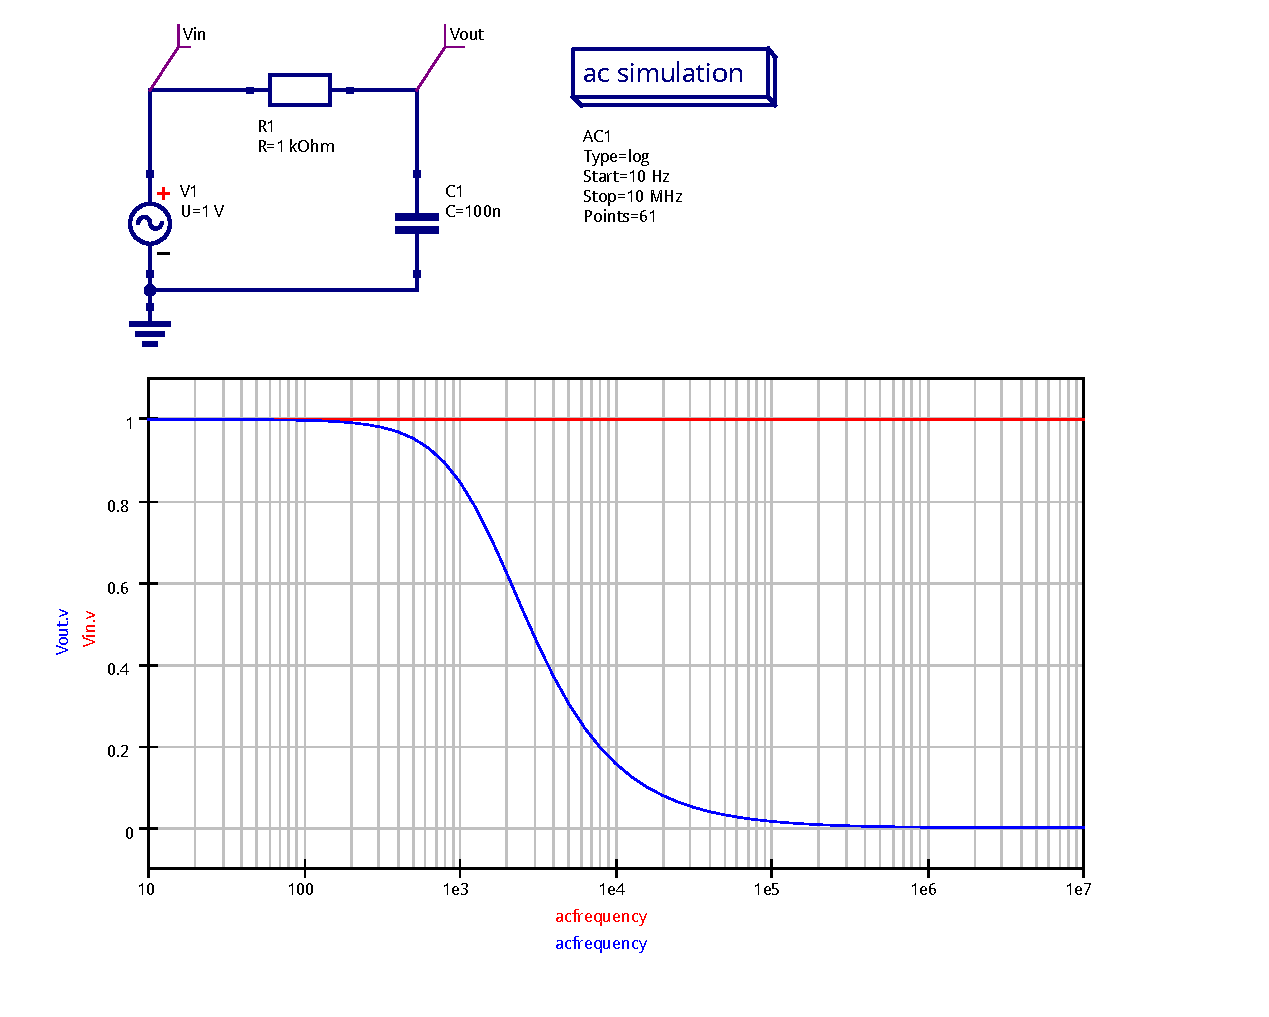
\includegraphics[width=\linewidth]{sim/ee466_lab-4_prj/uppgift-1_ac}
  \caption[] {Simulering av kretsens frekvensåtergivning.}
\end{figure}

\begin{figure}[ht]\label{fig:bode-sim-tran}
  \centering
  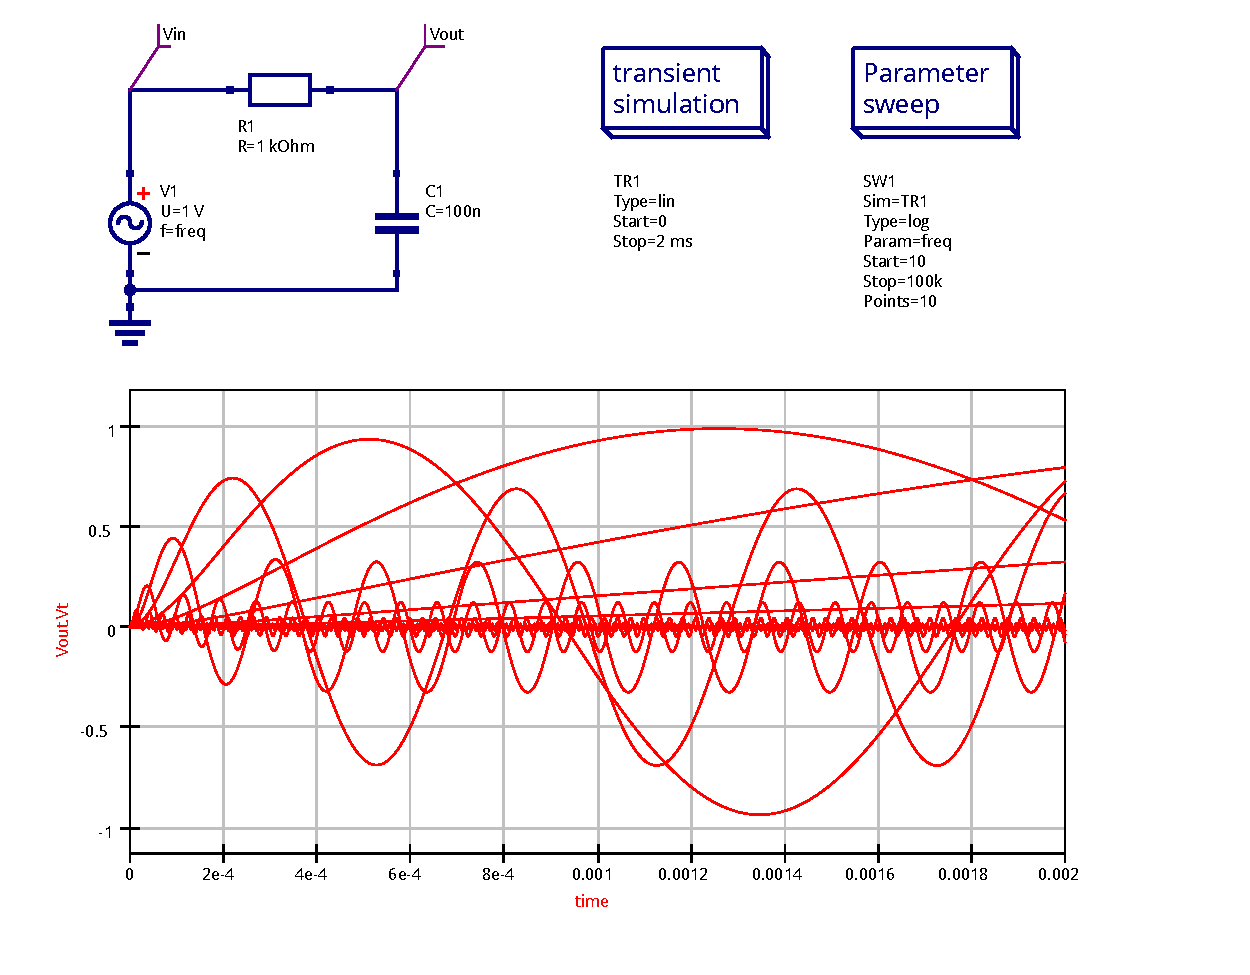
\includegraphics[width=\linewidth]{sim/ee466_lab-4_prj/uppgift-1_tran}
  \caption[] {Simulering av kretsen i tidsdomänen för olika frekvenser av $V_1$.}
\end{figure}

\begin{figure}[ht]\label{fig:bode-sim-param}
  \centering
  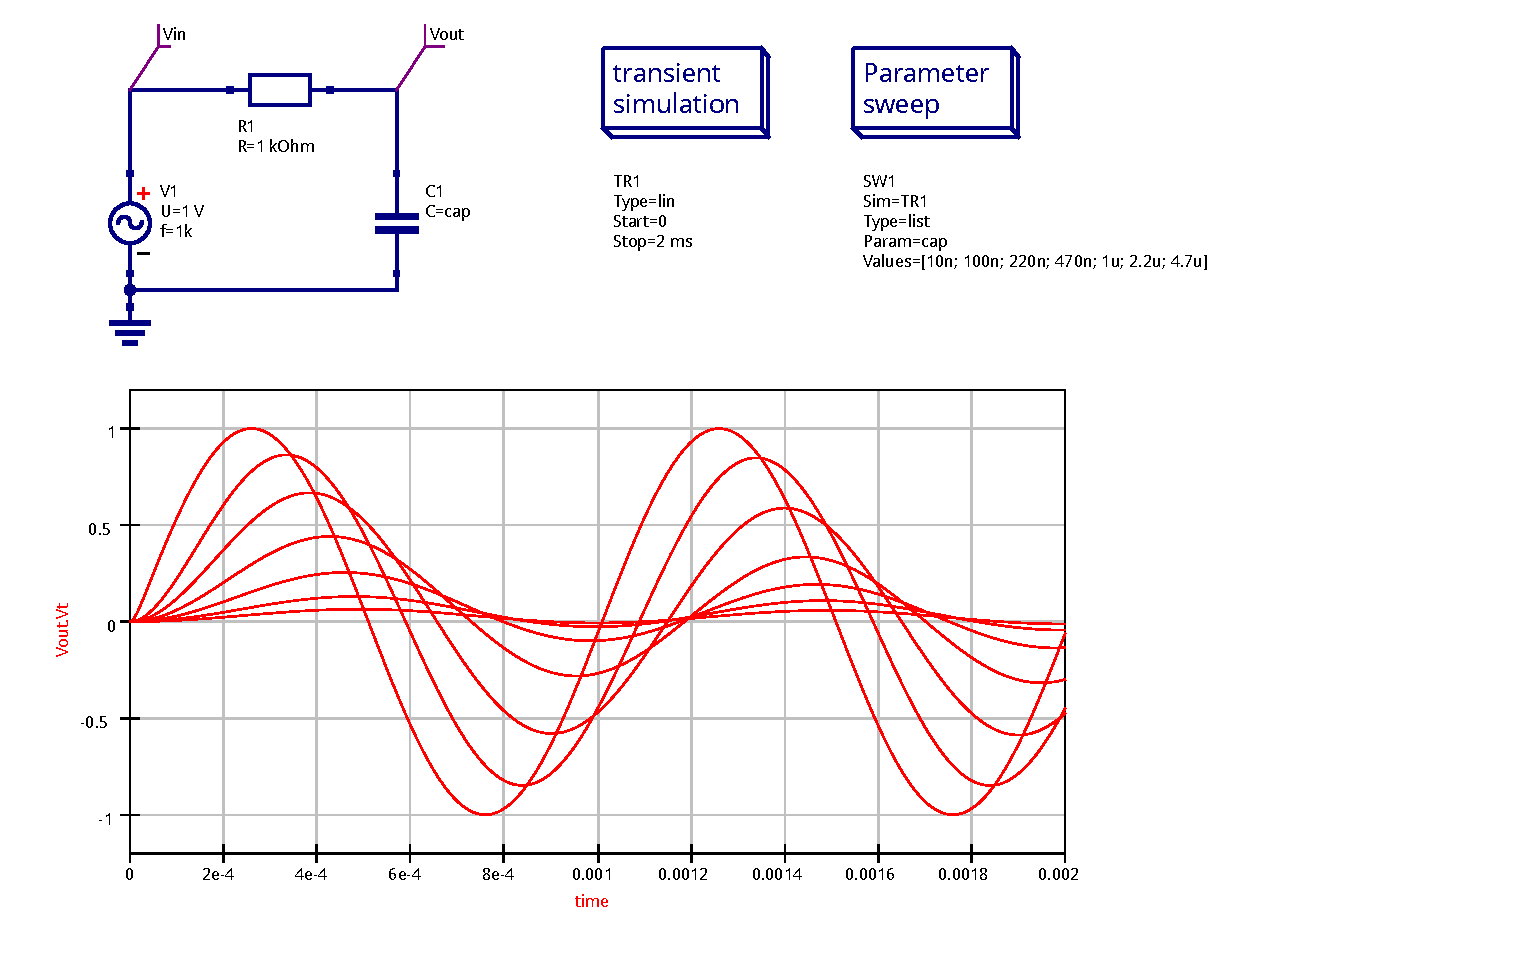
\includegraphics[width=\linewidth]{sim/ee466_lab-4_prj/uppgift-1_param}
  \caption[] {Simulering av kretsen i tidsdomänen för olika värden av $C_1$.}
\end{figure}


\subsection{Kommentar}\label{}
% ------------------------------------------------------------------------------
Mätresultaten ligger inom vad som kan antas vara rimligt för den använda
experimentuppställningen, komponenttoleranserna och mätutrustningens precision.
Den största förändringen sker inom ett begränsat frekvensområde vid och efter
brytfrekvensen. Med ett automatiserat test, med hjälp av programvara som t.ex.
\texttt{Labview} är det mer praktiskt genomförbart att göra utföra mätningar
med större precision och ett mycket större antal mätpunkter.


% ==============================================================================
% LAB 119
% UNDERSÖKNING AV RC-KRETS
% ------------------------
%
% Author:
% Jonas Sjöberg     <tel12jsg@student.hig.se>
% Oscar Wallberg    <tco13owg@student.hig.se>
%
% License:
% Creative Commons Attribution-NonCommercial-ShareAlike 4.0 International
% See LICENSE.md for full licensing information.
% ==============================================================================

\section{Uppmätning av stegsvaret}\label{step}
% ------------------------------------------------------------------------------
Stegsvaret mäts genom att kretsen matas med en fyrkantsvåg med en periodtid som
är tillräckligt lång för att utsignalen ($V_{out}$ i Figur~\ref{fig:rc-schema})
ska hinna uppnå sitt slutvärde för varje halvperiod.

% TODO: Graf för typiskt exponentiellt stegsvar.

Kretsens tidskonstant $\tau = RC$


\subsection{Mätresultat}\label{}
% ------------------------------------------------------------------------------
% TODO: Lägg till faktiska mätresultat för tidskonstant.
\begin{equation}
  \begin{split}
    \text{Uppmätt värde på } $\tau &= 1$             \\
    \text{Vilket ger } $f_1        &= 1 \si{\hertz}$ \\
  \end{split}
\end{equation}


\subsection{Simulering}\label{}
% ------------------------------------------------------------------------------
Kretsen simuleras i \texttt{Qucs} enligt Figur~\ref{fig:step-sim-step} och
Figur~\ref{fig:step-sim-param}.

Figur~\ref{fig:step-sim-step} visar det enkla fallet. En fyrkantsvåg används
för att illustrera hur kretsen svarar mot plötsliga förändringar. Grafen visar
spänningen vid punkten \texttt{Vout} som en funktion av tid.

Figur~\ref{fig:step-sim-param} visar samma skeende då värdet av $C_1$ sätts
till några av vanligt förekommande värden (standardiserade i \texttt{IEC
60063:1963}) genom en ''\emph{parameter sweep}``.  \par
Värden av $C_1$: \SI{10}{\nano\farad},  \SI{100}{\nano\farad},
                 \SI{220}{\nano\farad}, \SI{470}{\nano\farad},
                 \SI{1}{\micro\farad},  \SI{2.2}{\micro\farad}
             och \SI{4.7}{\micro\farad}.


\begin{figure}[ht]\label{fig:step-sim-step}
  \centering
  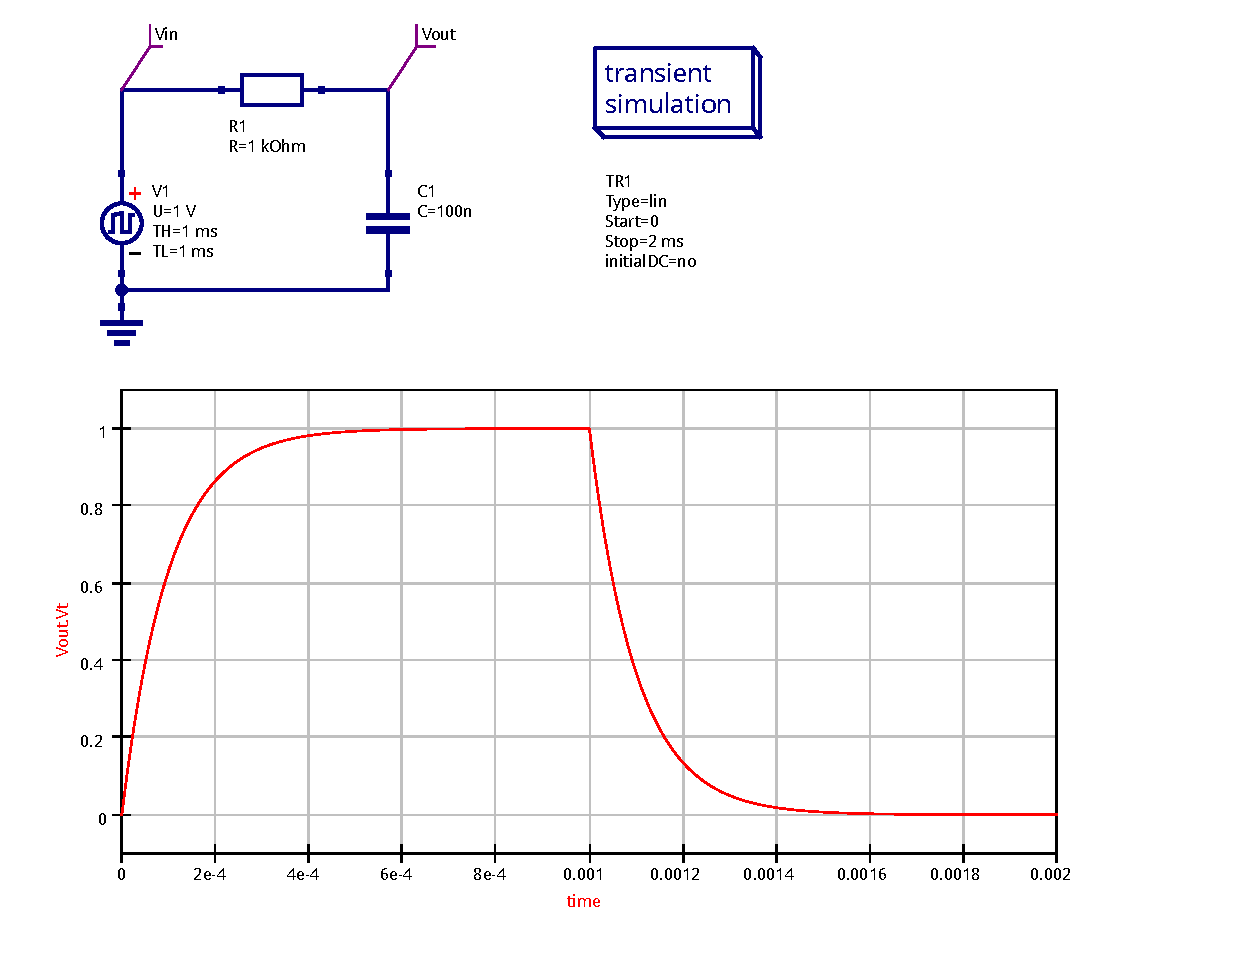
\includegraphics[width=\linewidth]{sim/ee466_lab-4_prj/uppgift-2_step}
  \caption[] {Simulering av kretsens stegsvar.}
\end{figure}

\begin{figure}[ht]\label{fig:step-sim-param}
  \centering
  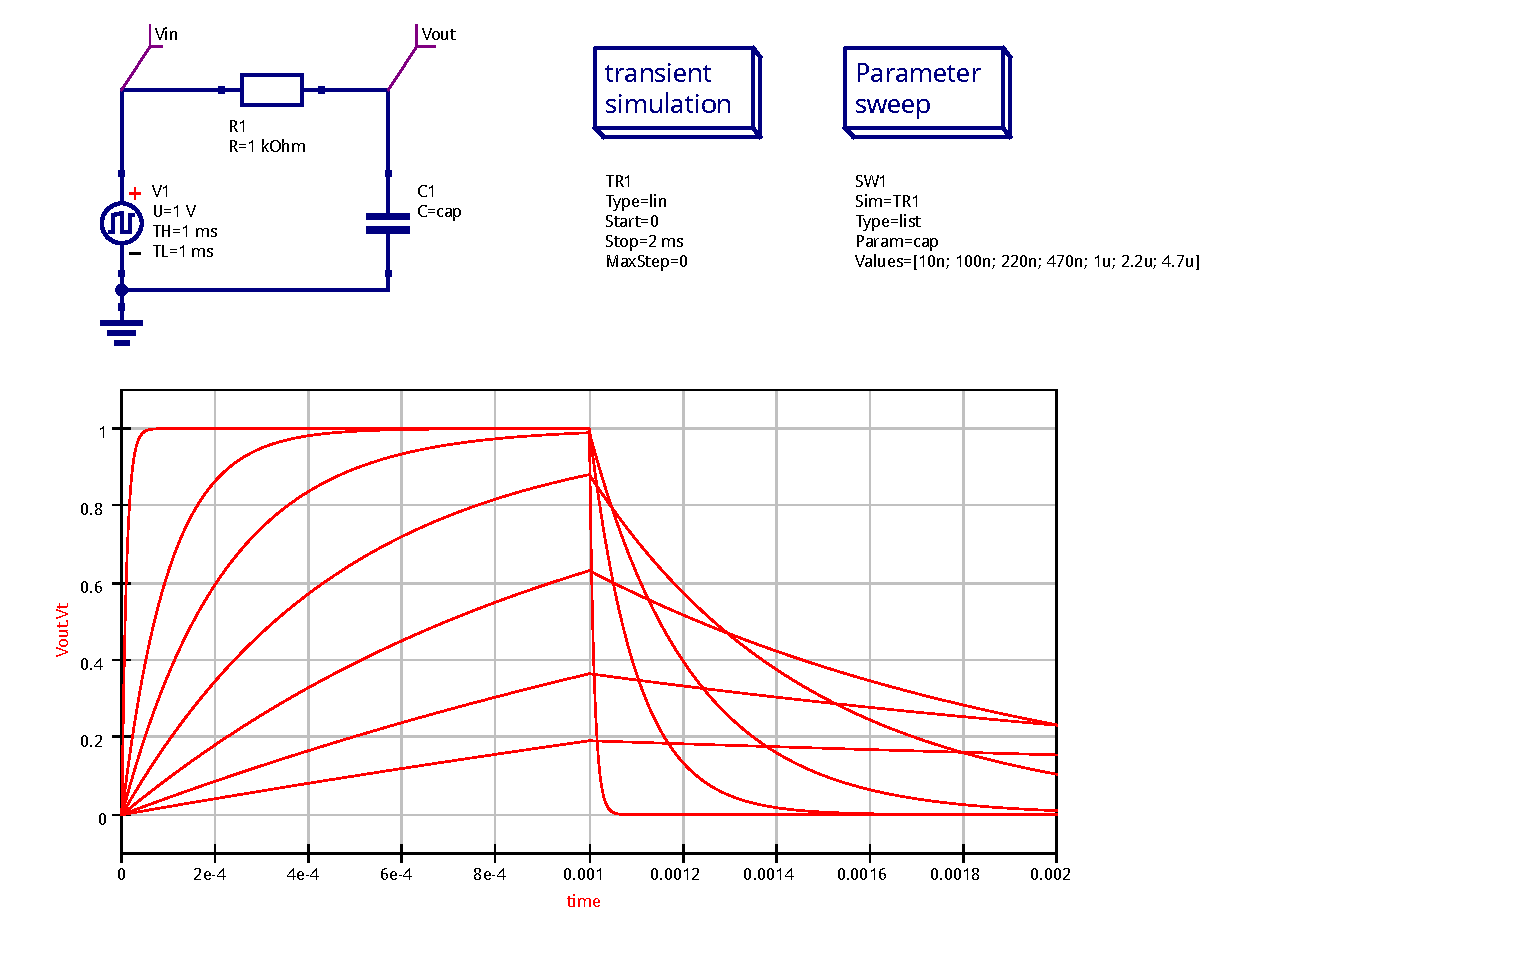
\includegraphics[width=\linewidth]{sim/ee466_lab-4_prj/uppgift-2_param}
  \caption[] {Simulering av kretsens stegsvar för olika värden av $C_1$.}
\end{figure}


\subsection{Kommentar}\label{}
% ------------------------------------------------------------------------------
% TODO: Hur stämmer deta uppmätta värdet av tidskonstanten med det beräknade
%       värdet och med det som erhölls ur Bode-diagrammet? 


% ==============================================================================
% LAB 119
% UNDERSÖKNING AV RC-KRETS
% ------------------------
%
% Author:
% Jonas Sjöberg     <tel12jsg@student.hig.se>
% Oscar Wallberg    <tco13owg@student.hig.se>
%
% License:
% Creative Commons Attribution-NonCommercial-ShareAlike 4.0 International
% See LICENSE.md for full licensing information.
% ==============================================================================

\section{Inverkan av källimpedans och belastningsimpedans}\label{impedans}
% ------------------------------------------------------------------------------
% Hittills har vi inte tagit hänsyn till hur signalgeneratorns och oscilloskopets
% impedanser kan påverka funktionen hos vår krets. Ett mera fullständigt schema
% över vår uppkoppling ser ut så här:
% 
% Om vi betraktar kondensatorn som kortsluten för höga frekvenser och som helt
% öppen för låga frekvenser så inser vi lätt att inimpedansen för RC-filtret Zin
% 1k och utimpedansen Zut 1k. Det är alltså rimligt att anta att varken
% signalgeneratorns eller oscilloskopets impedanser inverkar nämnvärt på kretsens
% funktion i vår uppkoppling.  Men vad händer om vi har käll- eller
% belastningsimpedanser i samma storleksordning som RC-kretsens egna impedanser?
% Vi kan undersöka detta genom att ansluta motstånd på in- och utgången av
% kretsen.

\section{Inverkan av källimpedansen}\label{Zin}
% ------------------------------------------------------------------------------
% För att se hur kretsen uppför sig om vi ansluter den till en signalgenerator
% med utimpedansen 1k (dvs egentligen 1k + 50) kopplar vi upp följande krets:

% TODO: Lägg till Kopplingsschema


\subsection{Mätresultat}\label{}
% ------------------------------------------------------------------------------
% TODO: Mät upp Bode-diagrammet för kretsen och jämför med tidigare fall, 
%       vi nöjer oss med amplituddiagrammet i denna mätning. 
%       Notera brytfrekvensen. 
%       Uin är den "nya" funktionsgeneratorns utspänning utan belastning.

% TODO: Lägg till signalgeneratorns amplitud vid mätning.
$U_{in} = 1 \si{\volt}$

% TODO: Lägg till faktiska mätresultat i tabellen.
\begin{longtable}[c]{@{}ccccc@{}}
  \toprule\addlinespace
    \begin{tabular}{cc}$\text{Frekvens}        \\ (\si{\hertz})$   \end{tabular}
  & \begin{tabular}{cc}$U_{ut}                 \\ (\si{\volt})$    \end{tabular}
  & \begin{tabular}{cc}$U_{ut}/U_{in}          \\ (\si{\volt})$    \end{tabular}
  & \begin{tabular}{cc}$20 \log{U_{ut}/U_{in}} \\ (\si{\dB})$      \end{tabular}
  \\\addlinespace
  \midrule\endhead
   100 & 2.11 & 1.01 & 5   \\\addlinespace
   200 & 2.06 & 0.99 & 10  \\\addlinespace
   300 & 2    & 0.96 & 17  \\\addlinespace
   500 & 1.94 & 0.93 & 24  \\\addlinespace
   700 & 1.84 & 0.88 & 29  \\\addlinespace
  1000 & 1.75 & 0.84 & 33  \\\addlinespace
  1200 & 1.66 & 0.79 & 37  \\\addlinespace
  1300 & 1.56 & 0.75 & 42  \\\addlinespace
  1500 & 1.49 & 0.71 & 45  \\\addlinespace
  1700 & 1.39 & 0.67 & 49  \\\addlinespace
  2000 & 1.39 & 0.67 & 49  \\\addlinespace
  \bottomrule
  \addlinespace
  \caption[]{Mätresultat för kretsen i Figur~\ref{fig:rc-schema}.}
  \label{8a-table}
\end{longtable}

% TODO: Bode-diagram för frekvensgång (amplitud vs frekvens).

% TODO: Hur påverkas amplituden och brytfrekvensen av källimpedansen? 


\section{Inverkan av belastningsimpedansen}\label{Zut}
% ------------------------------------------------------------------------------
% För att undersöka hur kretsen påverkas av en belastning på 1k kopplar vi upp
% följande:

% TODO: Lägg till Kopplingsschema


\subsection{Mätresultat}\label{}
% ------------------------------------------------------------------------------
% TODO: Mät upp amplituddiagrammet och notera brytfrekvensen.

% TODO: Lägg till signalgeneratorns amplitud vid mätning.
$U_{in} = 1 \si{\volt}$

% TODO: Lägg till faktiska mätresultat i tabellen.
\begin{longtable}[c]{@{}ccccc@{}}
  \toprule\addlinespace
    \begin{tabular}{cc}$\text{Frekvens}        \\ (\si{\hertz})$   \end{tabular}
  & \begin{tabular}{cc}$U_{ut}                 \\ (\si{\volt})$    \end{tabular}
  & \begin{tabular}{cc}$U_{ut}/U_{in}          \\ (\si{\volt})$    \end{tabular}
  & \begin{tabular}{cc}$20 \log{U_{ut}/U_{in}} \\ (\si{\dB})$      \end{tabular}
  \\\addlinespace
  \midrule\endhead
   100 & 2.11 & 1.01 & 5   \\\addlinespace
   200 & 2.06 & 0.99 & 10  \\\addlinespace
   300 & 2    & 0.96 & 17  \\\addlinespace
   500 & 1.94 & 0.93 & 24  \\\addlinespace
   700 & 1.84 & 0.88 & 29  \\\addlinespace
  1000 & 1.75 & 0.84 & 33  \\\addlinespace
  1200 & 1.66 & 0.79 & 37  \\\addlinespace
  1300 & 1.56 & 0.75 & 42  \\\addlinespace
  1500 & 1.49 & 0.71 & 45  \\\addlinespace
  1700 & 1.39 & 0.67 & 49  \\\addlinespace
  2000 & 1.39 & 0.67 & 49  \\\addlinespace
  \bottomrule
  \addlinespace
  \caption[]{Mätresultat för Inverkan av belastningsimpedansen för kretsen i Figur~\ref{fig:rc-schema}.}
  \label{8a-table}
\end{longtable}


% TODO: Bode-diagram för frekvensgång (amplitud vs frekvens).

% TODO: Hur påverkas amplituden och brytfrekvensen av belastningsimpedansen? 
%       Förklara vad som händer!



\subsection{Simulering}\label{}
% ------------------------------------------------------------------------------
Kretsen simuleras i \texttt{Qucs} enligt Figur~\ref{fig:Zin-step} och
Figur~\ref{fig:Zout-step}.

Källimpedansens påverkar på kretsen kan ses i Figur~\ref{fig:Zin-step} som
visar kretsens frekvensrespons då värdet av $R_i$ sveps mellan $\SI{50}{\ohm}$
och $\SI{10}{\kohm}$ i $20$ steg om $\SI{523.684}{\ohm}$.

Påverkan från belastningsimpedansen ses i Figur~\ref{fig:Zout-step} som visar
kretsens frekvensrespons då värdet av $R_o$ sveps mellan $\SI{100}{\ohm}$ och
$\SI{1}{\mega\ohm}$ i $101$ steg om $\SI{9.999}{\kohm}$.


\begin{figure}[ht]\label{fig:Zin-step}
  \centering
  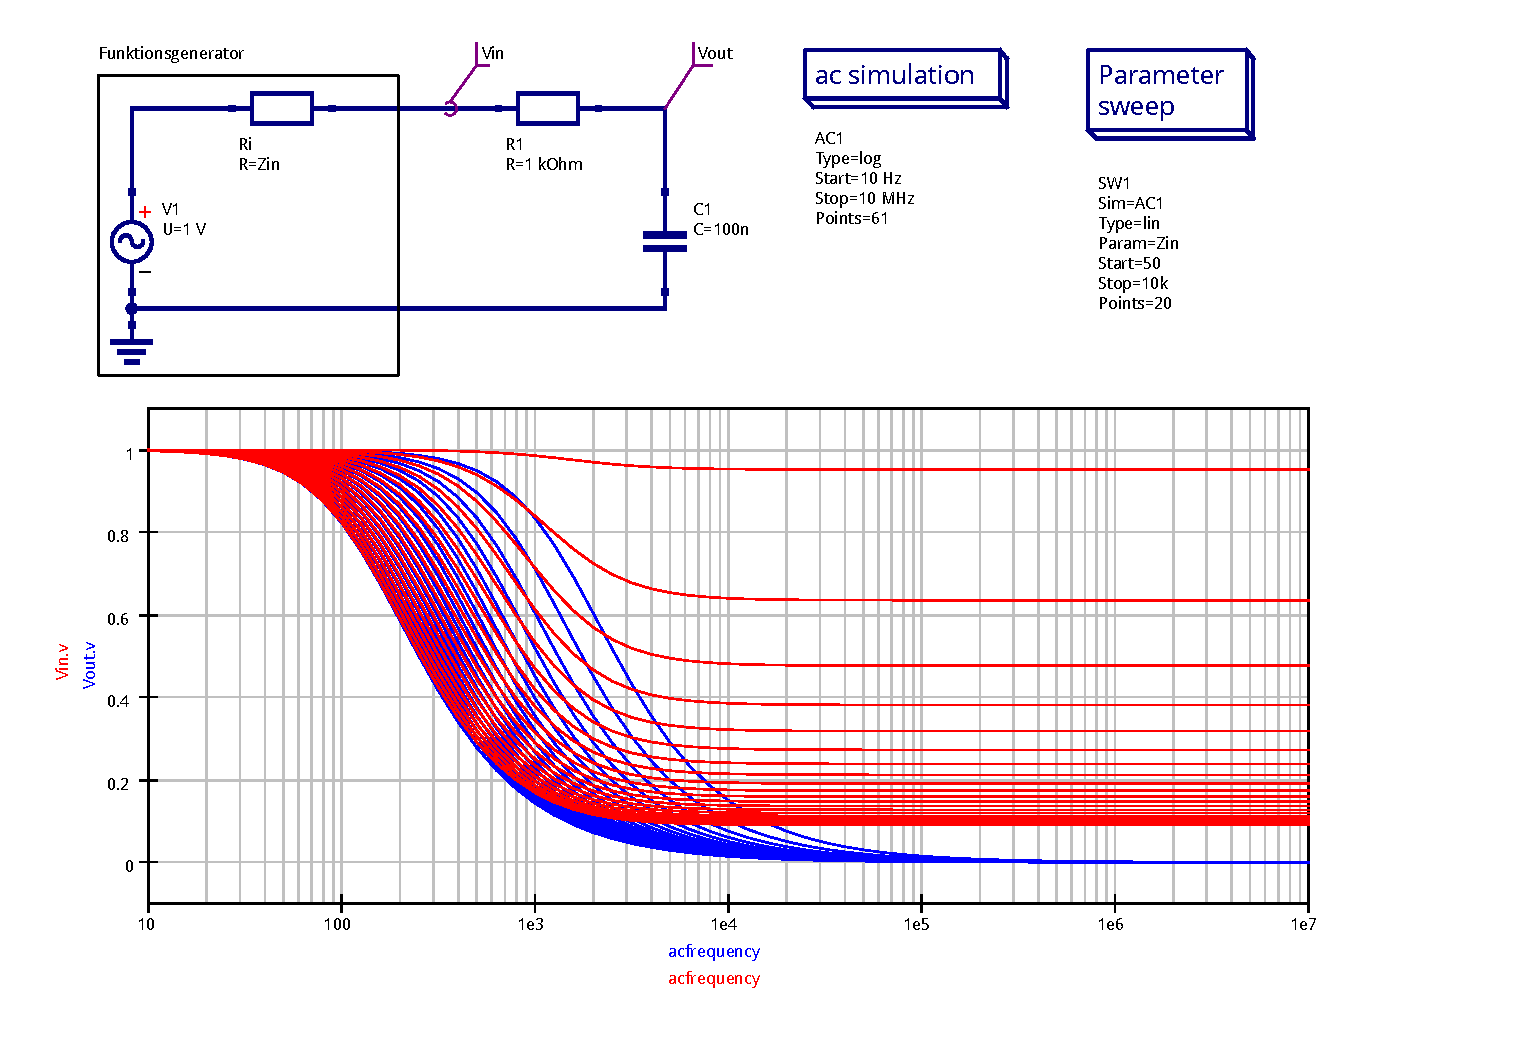
\includegraphics[width=\linewidth]{sim/ee466_lab-4_prj/uppgift-3_Zin_step}
  \caption[] {Simulering av kretsens frekvensrespons för olika värden av $R_i$.}
\end{figure}

\begin{figure}[ht]\label{fig:Zout-step}
  \centering
  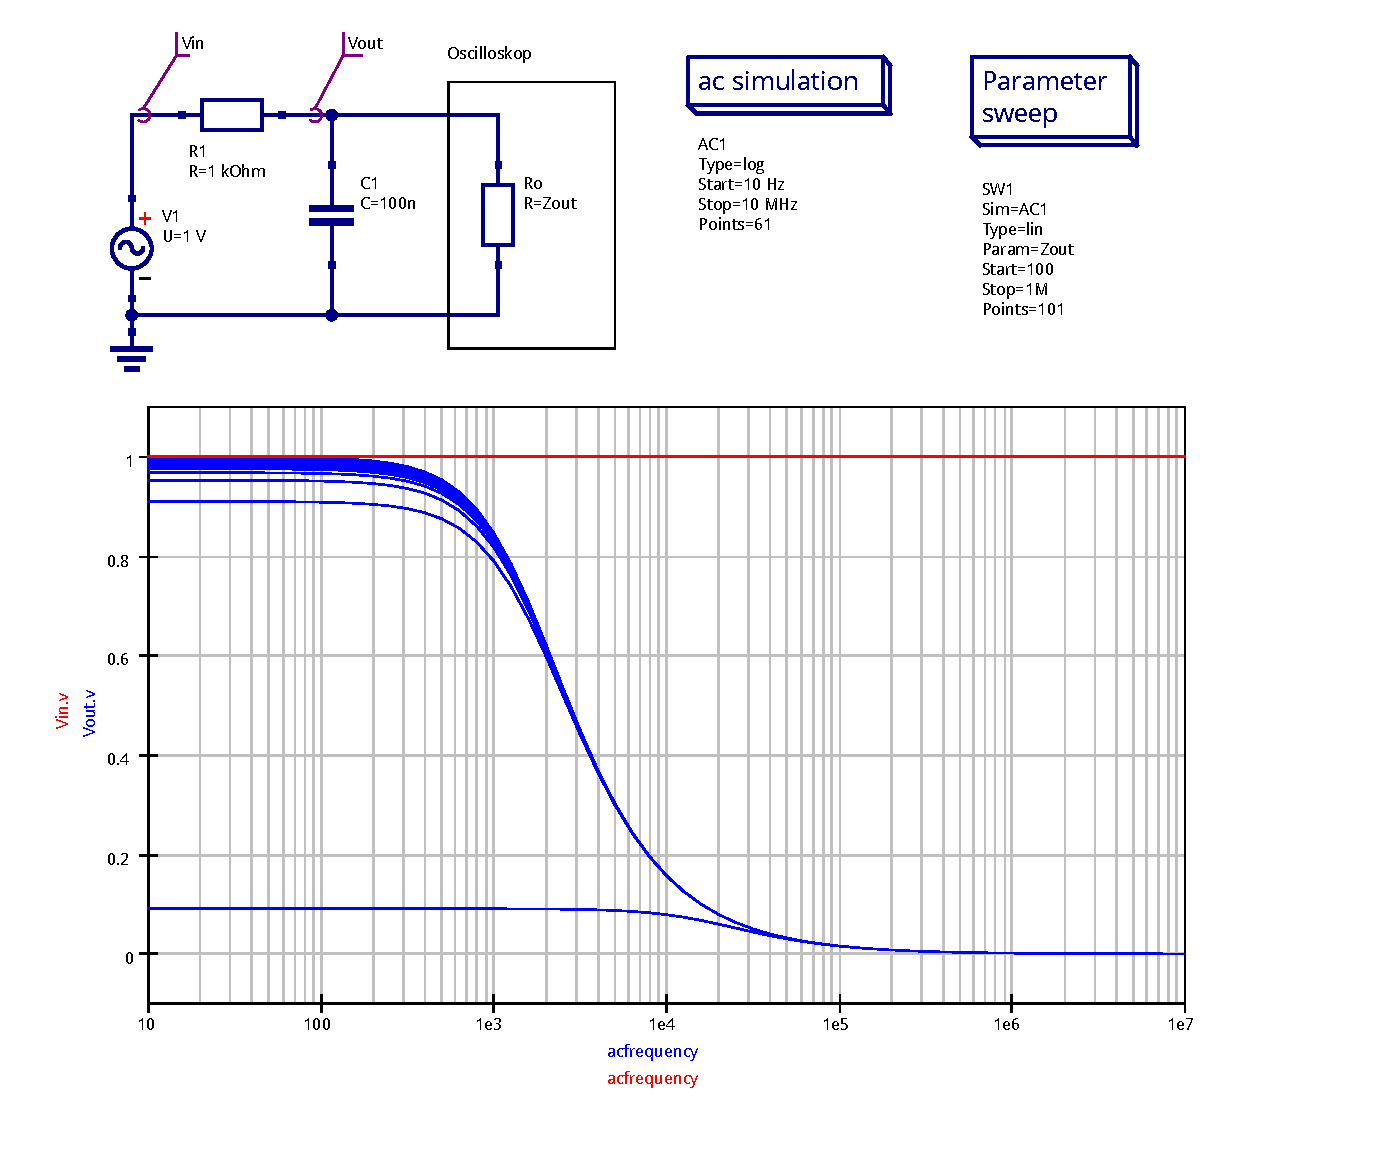
\includegraphics[width=\linewidth]{sim/ee466_lab-4_prj/uppgift-3_Zout_step}
  \caption[] {Simulering av kretsens frekvensrespons för olika värden av $R_o$.}
\end{figure}

\subsection{Kommentar}\label{}
% ------------------------------------------------------------------------------
% TODO:




\newpage
% ==============================================================================
% LAB 119
% UNDERSÖKNING AV RC-KRETS
% ------------------------
%
% Author:
% Jonas Sjöberg     <tel12jsg@student.hig.se>
%
% License:
% Creative Commons Attribution-NonCommercial-ShareAlike 4.0 International
% See LICENSE.md for full licensing information.
% ==============================================================================

\section{Resultat}\label{resultat}
% ------------------------------------------------------------------------------
Laborationen visar tydligt principer för kretsar av den typen. Då resultaten
avviker från de beräknade eller teoretiska antagandena kan förklaringar ges.
\par De problem jag stött på nämns i rapporten.

% ==============================================================================
% LAB 119
% UNDERSÖKNING AV RC-KRETS
% ------------------------
%
% Author:
% Jonas Sjöberg     <tel12jsg@student.hig.se>
%
% License:
% Creative Commons Attribution-NonCommercial-ShareAlike 4.0 International
% See LICENSE.md for full licensing information.
% ==============================================================================

\section{Referenser}\label{refs}
% ------------------------------------------------------------------------------
%TODO: Referenser.

%\subsection{www}\label{interwebs}
% ------------------------------------------------------------------------------

%\subsection{Trycksaker}\label{literature} %???
% ------------------------------------------------------------------------------

\subsection{Källkod}\label{sourcefiles}
% ------------------------------------------------------------------------------
Källkod till rapporten med alla arbetsfiler till \texttt{SPICE}-simuleringen
finns tillgängliga på \url{https://github.com/jonasjberg/EE466-lab04}
\par Hämta hem repon genom att exekvera följande från kommandoraden:
\begin{verbatim}
> $ git clone git@github.com:jonasjberg/DVG303_lab3.git
\end{verbatim}




\end{document}
